\subsection{Parametrizations of Affine Varieties}


\begin{exercise}{4}
Consider the parametric representation
\begin{align*}
    x=\frac{t}{1+t},\,\,y=1-\frac{1}{t^2}.
\end{align*}
\begin{enumerate}
    \item Find the equation of the affine variety determined by the above parametric equations.
    \item Show that the above equations parametrize all points of the variety found in part (1) except for the point $(1,1)$.
\end{enumerate}
\end{exercise}
\begin{proof}
\begin{enumerate}
    \item We have 
    \begin{align*}
        &x = \frac{t}{1+t}\iff\\
        &x(1+t) = t\iff\\
        &x = t(1-x)\iff\\
        &t = \frac{x}{1-x},
    \end{align*}
    so that replacing in the equation of $y$ we obtain the equation of the affine variety
    \begin{align*}
        y =& 1 -\frac{1}{\left(\frac{x}{1-x}\right)^2}\\
        =& 1-\frac{(1-x)^2}{x^2}\\
        =& \frac{x^2-1+2x-x^2}{x^2}\iff\\
        &yx^2-2x+1=0.
    \end{align*}
    \item To show this, we simply replace the parametrised equation for $x$ and $y$ in the equation of the affine variety
    \begin{align*}
        &\parens{1-\frac{1}{t^2}}\parens{\frac{t}{1+t}}^2-2\parens{\frac{t}{1+t}}+1=0\\
        &\parens{\frac{t^2(t^2-1)}{t^2(1+t)^2}}-2\parens{\frac{t^3(1+t)}{t^2(1+t)^2}}+1=0\\
        &\parens{\frac{t^4-t^2-2t^3-2t^4}{t^2(1+t)^2}}+1=0\\
        &\frac{t^4-t^2-2t^3-2t^4+t^2(1+t)^2}{t^2(1+t)^2}=0\\
        &\frac{t^4-t^2-2t^3-2t^4+t^2(1+2t+t^2)}{t^2(1+t)^2}=0\\
        &\frac{t^4-t^2-2t^3-2t^4+t^2+2t^3+t^4)}{t^2(1+t)^2}=0\\
        &0=0.
    \end{align*}
    Notice, however, that if $x=1$, then $1=t/(1+t)$ so that $1+t=t$ which is a contradiction.
\end{enumerate}
\end{proof}

\begin{exercise}{6}
The goal of this problem is to show that the sphere $x^2+y^2+z^2=1$ in 3-dimensional space can be parametrised by
\begin{align*}
    x=\frac{2u}{u^2+v^2+1},\,\, y=\frac{2v}{u^2+v^2+1},\,\, z=\frac{u^2+v^2-1}{u^2+v^2+1}.
\end{align*}
The idea is to adapt the argument used for the circle $x^2+y^2=1$ to 3-dimensional space.
\begin{enumerate}
    \item Given a point $(u,v,0)$ in the $(x,y)$-plane, draw the line form this point to the ``north pole'' $(0,0,1)$ of the sphere, and let $(x,y,z)$ be the other point where the line meets the sphere. Draw a picture to illustrate this, and argue geometrically that mapping $(u,v)$ to $(x,y,z)$ gives a parametrisation of the sphere minus the north pole.
    \item Show that the line connecting $(0,0,1)$ to $(u,v,0)$ is parametrised by $(tu,tv,1-t)$, where $t$ is a parameter that moves along the line.
    \item Substitute $x=tu, y=tv$ and $z=1-$ into the equation for the sphere $x^2+y^2+z^2=1$. Use this to derive the formulas given at the beginning of the problem.
\end{enumerate}
\end{exercise}
\begin{proof}
fill
\end{proof}

\begin{exercise}{8}
Consider the curve defined by $y^2=cx^2-x^3$, where $c$ is some constant. Here is a picture of the curve when $c>0$:
\begin{figure}[H]
     \centering
     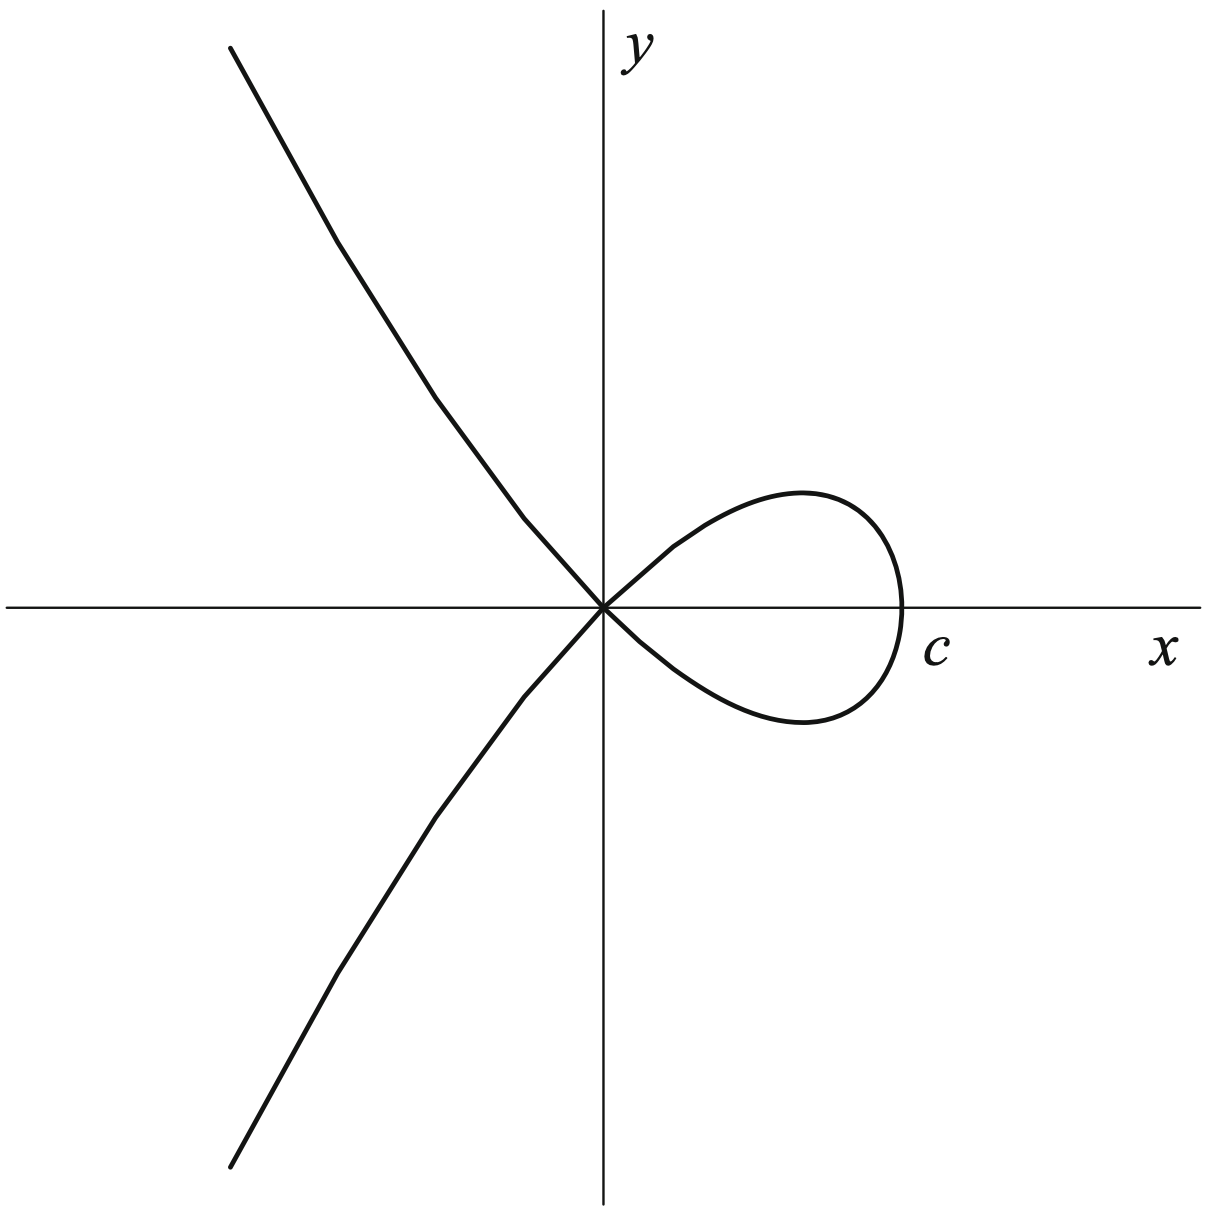
\includegraphics[width=.5\textwidth]{cox-little-oshea/assets/sec1-3-ex8.png}
     \caption{Fill}
     \label{fig:sec1-2-ex8}
\end{figure}
Our goal is to parametrise this curve.
\begin{enumerate}
    \item Show that a line will meet this curve at either 0, 1, 2, or 3 points. Illustrate your answer with a picture. Hint: let the equation of the line be either $x=a$ or $y=mx+b$.
    \item Show that a nonvertical line through the origin meets the curve at exactly on other point when $m^2\neq c$. Draw a picture to illustrate this, and see if you can come up with an intuitive explanation as to why this happens.
    \item Now draw the vertical line $x=1$. Given a point $(1,t)$ on this line, draw the line connecting $(1,t)$ to the origin. This will intersect the curve in a point $(x,y)$. Draw a picture to illustrate this, and argue geometrically that this gives a parametrisation of the entire curve.
    \item Show that the geometric description from part (3) leads to the parametrisation $x=c-t^2, y=t(c-t^2)$. 
\end{enumerate}
\end{exercise}
\begin{proof}
fill
\end{proof}

\begin{exercise}{11}
In this problem, we will derive the paramtrisation
\begin{align*}
    x = t(u^2-t^2),\,\, y = u,\,\, z = u^2-t^2
\end{align*}
of the surface $x^2-y^2z^2+z^3=0$ considered in the text.
\begin{enumerate}
    \item Adapt the formulas in part (4) of exercise 8 to show that the curve $x^2 = cz^2-z^3$ is parametrized by 
    \begin{align*}
        z=c-t^2,\,\, x=t(c-t^2).
    \end{align*}
    \item Now replace the c in part (1) by $y^2$, and explain how this leads to the above parametrisation of $x^2-y^2z^2+z^3=0$.
    \item Explain why this parametrisation covers the entire surface $\bV(x^2-y^2z^2+z^3$. Hint: See part (3) of exercise 8.
\end{enumerate}
\end{exercise}
\begin{proof}
fill
\end{proof}
